% Created 2020-09-18 Fri 17:13
% Intended LaTeX compiler: pdflatex
\documentclass[presentation]{beamer}
\usepackage[utf8]{inputenc}
\usepackage[T1]{fontenc}
\usepackage{graphicx}
\usepackage{grffile}
\usepackage{longtable}
\usepackage{wrapfig}
\usepackage{rotating}
\usepackage[normalem]{ulem}
\usepackage{amsmath}
\usepackage{textcomp}
\usepackage{amssymb}
\usepackage{capt-of}
\usepackage{hyperref}
\usetheme{UoB}
\author{Mark Blyth}
\date{\textit{[2020-09-21 Mon]}}
\title{Papers, splines, and other ideas}
\hypersetup{
 pdfauthor={Mark Blyth},
 pdftitle={Papers, splines, and other ideas},
 pdfkeywords={},
 pdfsubject={},
 pdfcreator={Emacs 27.1 (Org mode 9.3)}, 
 pdflang={English}}
\begin{document}

\maketitle

\section{Background}
\label{sec:orga553dc9}
\begin{frame}[label={sec:org79733a5}]{Presentation overview}
\begin{itemize}
\item Splines discretisation progress
\end{itemize}
\vfill
\begin{itemize}
\item Some ideas: projects that will enhance CBC, and make it more powerful for studying neurons
\begin{itemize}
\item Lots of exciting ideas; these ones are limited to the project-relevant ones
\end{itemize}
\end{itemize}
\end{frame}


\section{Splines discretisation progress}
\label{sec:orgc0c9dae}
\begin{frame}[label={sec:org64fd17c}]{CBC code progress}
\begin{itemize}
\item Rewritten for a new solver
\item Works for Fourier
\end{itemize}

\begin{center}
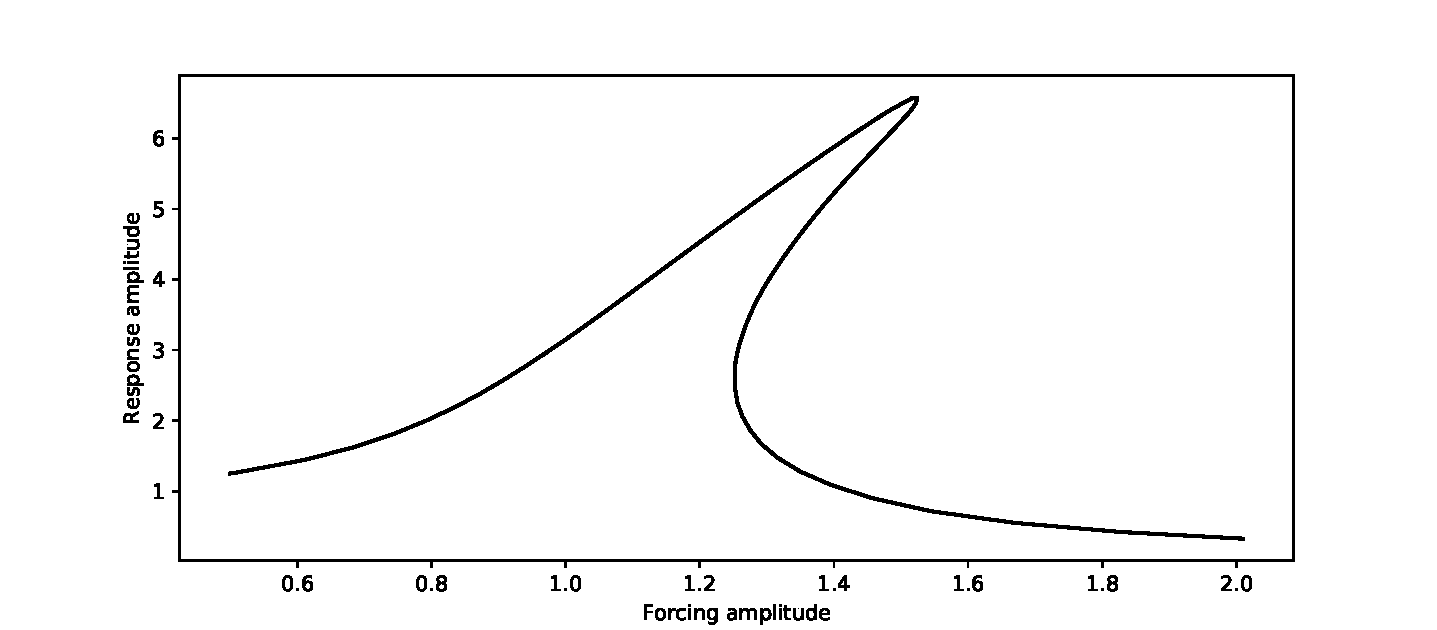
\includegraphics[width=.9\linewidth]{./newcode.pdf}
\end{center}
\end{frame}

\begin{frame}[label={sec:org2c450ec}]{Splines discretisation progress}
\begin{itemize}
\item Newton iterations fail to converge with splines discretisation
\end{itemize}
\vfill
\begin{itemize}
\item Working hypothesis: splines models are structurally unstable; small perturbations cause big changes
\begin{itemize}
\item Finite differences evaluates gradients by using small perturbations
\item Finite differences perturbations lead to discontinuous changes in the model
\end{itemize}
\end{itemize}
\end{frame}


\begin{frame}[label={sec:org81c153f}]{Splines discretisation progress}
\begin{center}
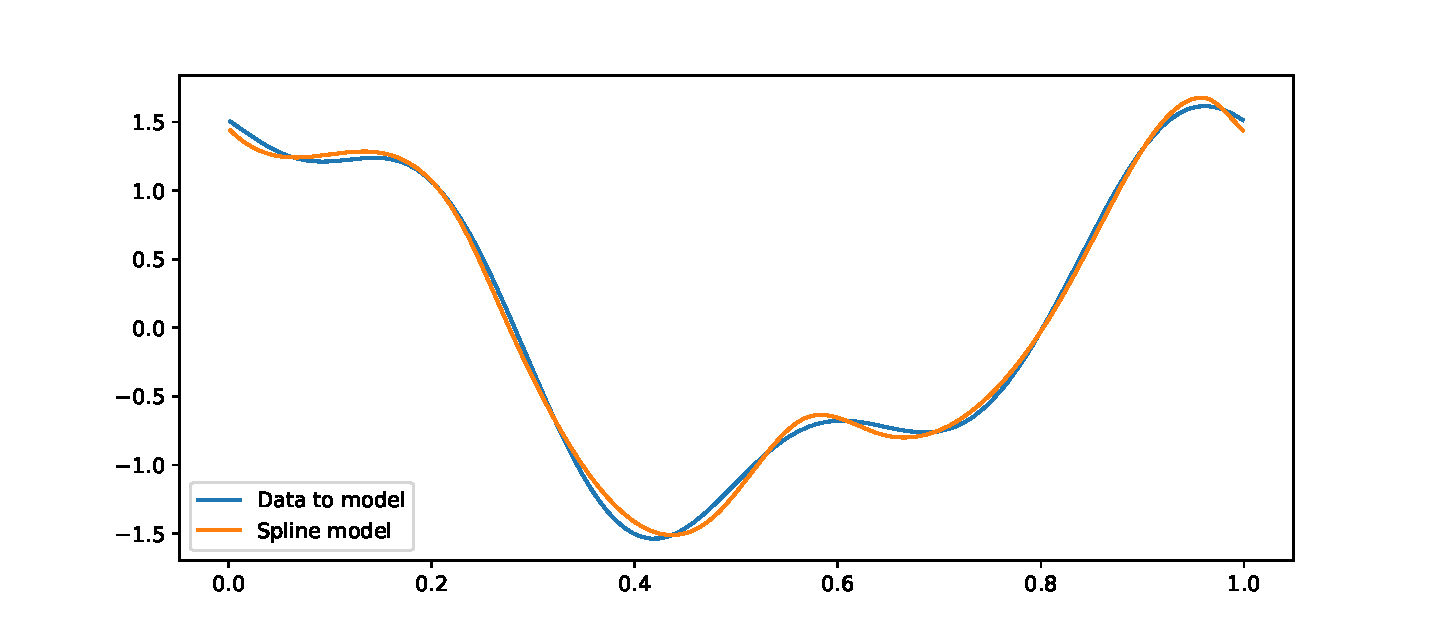
\includegraphics[width=.9\linewidth]{./modelling.pdf}
\end{center}

Spline model describes data fairly accurately
\end{frame}

\begin{frame}[label={sec:org8c27617}]{Splines discretisation progress}
\begin{center}
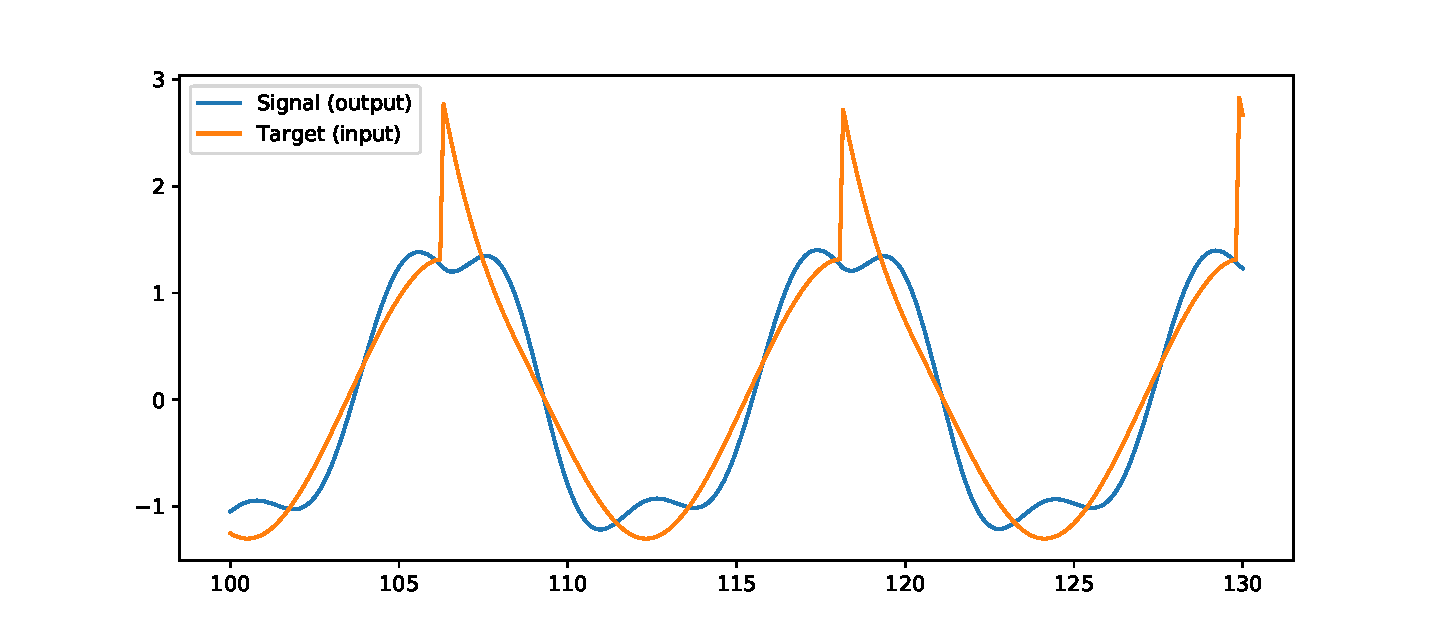
\includegraphics[width=.9\linewidth]{./perturbation.pdf}
\end{center}

Control-target input is discontinuous during Jacobian estimation
\end{frame}

\begin{frame}[label={sec:org024bc59}]{Splines discretisation progress}
\begin{itemize}
\item Newton iterations fail to converge with splines discretisation
\end{itemize}
\vfill
\begin{itemize}
\item Working hypothesis: splines models are structurally unstable; small perturbations cause big changes
\begin{itemize}
\item Finite differences evaluates gradients by using small perturbations
\item Finite differences perturbations lead to discontinuous changes in the model
\end{itemize}
\end{itemize}
\vfill
\begin{itemize}
\item Currently a best-guess conjecture
\begin{itemize}
\item Need to play about more to see if this is actually the case
\item Need to test different finite-differences stepsizes
\end{itemize}
\end{itemize}
\end{frame}


\section{Project ideas}
\label{sec:orgeeeae7d}
\begin{frame}[label={sec:orga88abc4}]{Novel discretisors}
Ideal: journal paper comparing\ldots{}
\vfill
\begin{itemize}
\item Splines
\begin{itemize}
\item Knot selection methods?
\end{itemize}
\item Wavelets
\item Collocation
\item Fourier
\end{itemize}

\vfill
Compare for noise-robustness, dimensionality, computational speed
\end{frame}

\begin{frame}[<+->][label={sec:org0161f49},plain]{Idea 1: Extended novel discretisors}
\begin{itemize}
\item Extension 1 [discussed in meetings]: selecting discretisation method based on model evidence
\begin{itemize}
\item Produce Bayesian inference method for Fourier harmonics
\item Replace `simple' splines / wavelets / collocation with Bayesian alternative
\item `Intelligently' select the best discretisor
\end{itemize}
\end{itemize}
\vfill
\begin{itemize}
\item Extension 2: reversible-jump MCMC for Fourier model identification
\begin{itemize}
\item Automatically determine best number of Fourier harmonics for any given signal
\item Similar to how BARS auto-chooses knot numbers and locations, but instead Fourier harmonics
\end{itemize}
\end{itemize}
\vfill
\begin{itemize}
\item Why Bayesian?
\begin{itemize}
\item Automatic Occam's razor
\item Optimally balances goodness-of-fit against model complexity; ensures simplest, most generalizable discretisations; statistically optimal
\end{itemize}
\end{itemize}
\end{frame}

\begin{frame}[label={sec:orge069ffd},plain]{The sweetspot problem}
\begin{center}
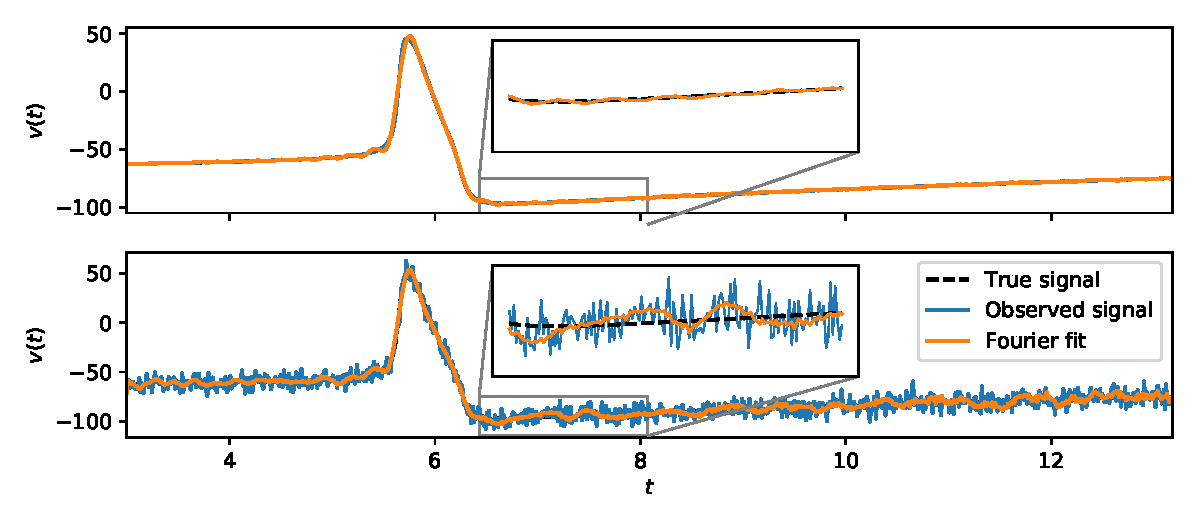
\includegraphics[width=.9\linewidth]{./fourier_demo.pdf}
\end{center}

\begin{itemize}
\item Sweetspot problem: too few harmonics don't fit; too many harmonics overfit noise
\item Bayesian Fourier model selection would find the sweet spot by automatically trading goodness-of-fit against model complexity
\end{itemize}
\end{frame}

\begin{frame}[<+->][label={sec:orgb85d4ca},plain]{Idea 2: discretisation-free CBC}
\begin{itemize}
\item As removed from NODYCON abstract
\begin{itemize}
\item Project surrogate of system output onto fundamental harmonic
\item Subtract out surrogate's fundamental harmonic
\item Replace fundamental harmonic with harmonic forcing term
\item Feed the modified surrogate back into the system as the new control target
\end{itemize}
\end{itemize}
\vfill
\begin{itemize}
\item Should converge rapidly, implicitly represent an infinite number of harmonics, improve computational speed by avoiding DFT, improve noise-robustness by employing surrogate noise-filtering
\end{itemize}

\vfill
\begin{itemize}
\item Further extension: something resembling a Picard iteration
\end{itemize}
\end{frame}

\begin{frame}[<+->][label={sec:org0a3e166},plain]{Idea 3: noise-robust numerical solvers}
\begin{itemize}
\item CBC strategies solve for input=output
\begin{itemize}
\item Harder to solve if output is corrupted by noise, or subject to stochastic dynamics -- both prevalent with neurons
\item `True' stochasticity -- measurement noise means evaluating the IO map for the same input won't necessarily give the same output
\item How do we decide when we've found a solution to a system, if the system is stochastic?
\item How do we decide if input\(\neq\) output because we haven't converged, or just because of noise?
\end{itemize}
\end{itemize}
\vfill
\begin{itemize}
\item Solver approach: input - output = 0
\item Minimizer approach: find input that minimizes (input - output)\textsuperscript{2}
\item These two approaches are identical in the noise-free case
\begin{itemize}
\item Control target is a solution to one if and only if it's a solution to the other
\end{itemize}
\item Minimizer approach is better in the noisy case
\begin{itemize}
\item If the system is subject to noise or stochastics, output will never truly equal input
\item Noninvasive solution will therefore minimize control action \emph{[minimizer works]}, but will not result in input-output=0 \emph{[solver won't work]}
\item Bonus: \emph{lots} of research on stochastic gradient descent (stochastic optimization) to help with this
\end{itemize}
\item Research output: comparison of convergence time, noise-robustness for minimization approach, solver approach
\end{itemize}
\end{frame}

\begin{frame}[<+->][label={sec:orgddc6ff7},plain]{Idea 4: alternative noise-robust numerical solvers}
\begin{itemize}
\item Covers same issues as before, but in a different way
\begin{itemize}
\item How do we decide when we've found a solution to a system, if the system is stochastic?
\item How do we decide if input\(\neq\) output because we haven't converged, or just because of noise?
\end{itemize}
\end{itemize}
\vfill
\begin{itemize}
\item Newton iterations are slow, even with Jacobian updates
\begin{itemize}
\item Especially big issue for larger-dimensional discretisations (as with neurons!)
\end{itemize}
\item IDEA: surrogates-based approach
\begin{itemize}
\item Build a surrogate of the input\(\to\)output map
\item Choose next function evaluation based on knowledge-gradient or expected improvement
\item With a probabilistic approach, this should converge much faster than Newton, and in a noise-robust way
\item Use a splines model for the input-output map, as GPR doesn't handle MIMO well
\item Extension of Barton-Renson conference paper: uses explicit MIMO models, knowledge gradients, explicit noise modelling
\end{itemize}
\item Aim main paper at a numerical methods audience; possibly additional journal paper comparing CBC speeds, noise-robustnesses for various numerical solvers
\end{itemize}
\end{frame}


\begin{frame}[<+->][label={sec:org5585dd5},plain]{Results}
\begin{itemize}
\item Efficient discretisation methods
\begin{itemize}
\item Alternative approaches to Fourier (splines, collocation, wavelets)
\item Allows the discretisation of spiking, neuron-like signals
\end{itemize}
\end{itemize}
\vfill
\begin{itemize}
\item Intelligent discretisation methods
\begin{itemize}
\item Bayesian'ly determine the best discretisor class \emph{[eg. Fourier vs. splines]}, best discretisation approach within that class \emph{[eg. number of knots / harmonics]}
\item Allows the optimal discretisation of spiking, neuron-like signals, without needing a human in the loop
\item Ensures CBC is accurate, by guaranteeing discretisation actually describes the target signal
\end{itemize}
\end{itemize}
\vfill
\begin{itemize}
\item Noise-robust solvers for accurate CBC calculations
\begin{itemize}
\item Solve the CBC equations accurately, even faced with measurement noise \emph{[and stochasticity?]}
\end{itemize}
\end{itemize}
\vfill
These produce a neuron-capable continuation procedure; paired with a control strategy, they'll allow neuronal CBC
\end{frame}

\begin{frame}[label={sec:orgfc37b0f}]{Testing the new methods}
Any CBC rigs I could demonstrate these methods on?
\end{frame}

\section{Next steps}
\label{sec:org43dd424}
\begin{frame}[label={sec:org822b81d}]{Next steps}
\begin{itemize}
\item Edit NODYCON paper
\item Edit continuation paper
\item Keep working on splines discretisation code
\item Test other discretisor methods
\end{itemize}
\end{frame}
\end{document}
